\begin{figure*}[h]
\begin{subfigure}{0.24\linewidth}
\centering
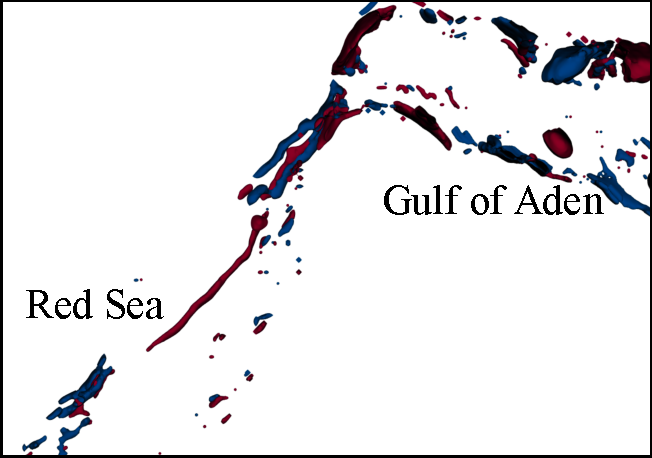
\includegraphics[width=\linewidth]{Images/RedSeaEddy/zls.pdf}
\caption{$ZLS_{T}$}
\label{}
\end{subfigure}
\begin{subfigure}{0.24\linewidth}
\centering
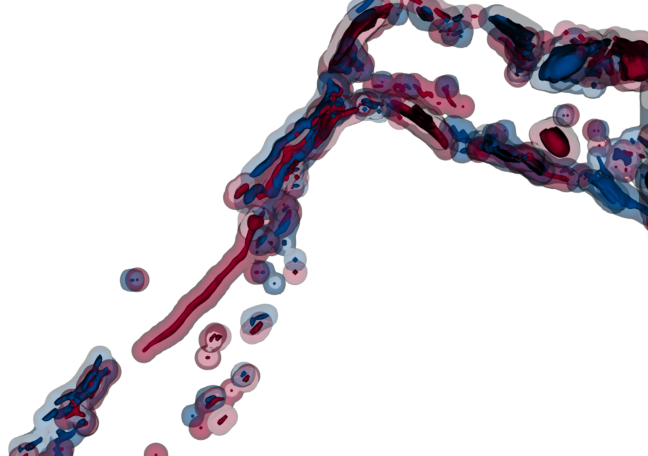
\includegraphics[width=\linewidth]{Images/RedSeaEddy/fls_6.pdf}
\caption{$ZLS_{T}$ + $FLS_{T,6}$}
\label{}
\end{subfigure}
\begin{subfigure}{0.24\linewidth}
\centering
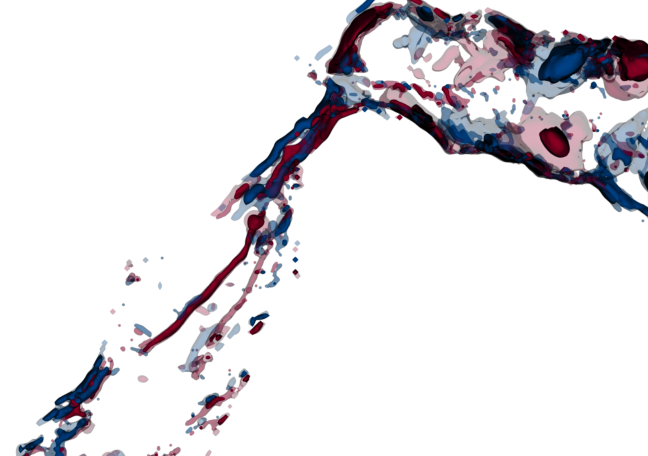
\includegraphics[width=\linewidth]{Images/RedSeaEddy/fcls_68.pdf}
\caption{$ZLS_{T}$ + $FCLS_{T,68\%}$}
\label{}
\end{subfigure}
\begin{subfigure}{0.24\linewidth}
\centering
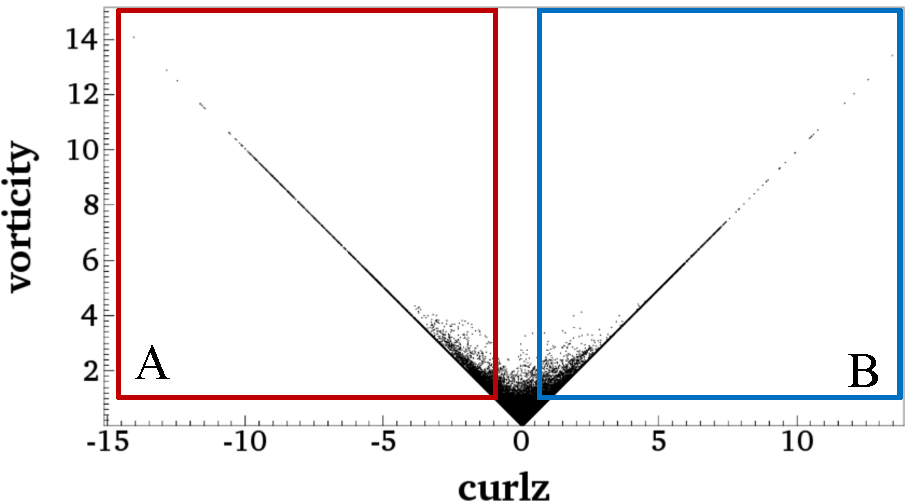
\includegraphics[width=0.95\linewidth]{Images/RedSeaEddy/scatterplot.pdf}
\caption{Attribute space 2D scatterplot and, traits (labeled rectangular selections). We use $T = \left\{T_{A}, T_{B}\right\}$.} 
\label{}
\end{subfigure}
\caption{}
\label{}
\end{figure*}
